% Auto-generated LaTeX figure snippets for Complex Networks 2026 paper



% ============================================================\begin{figure}[t!]
\centering
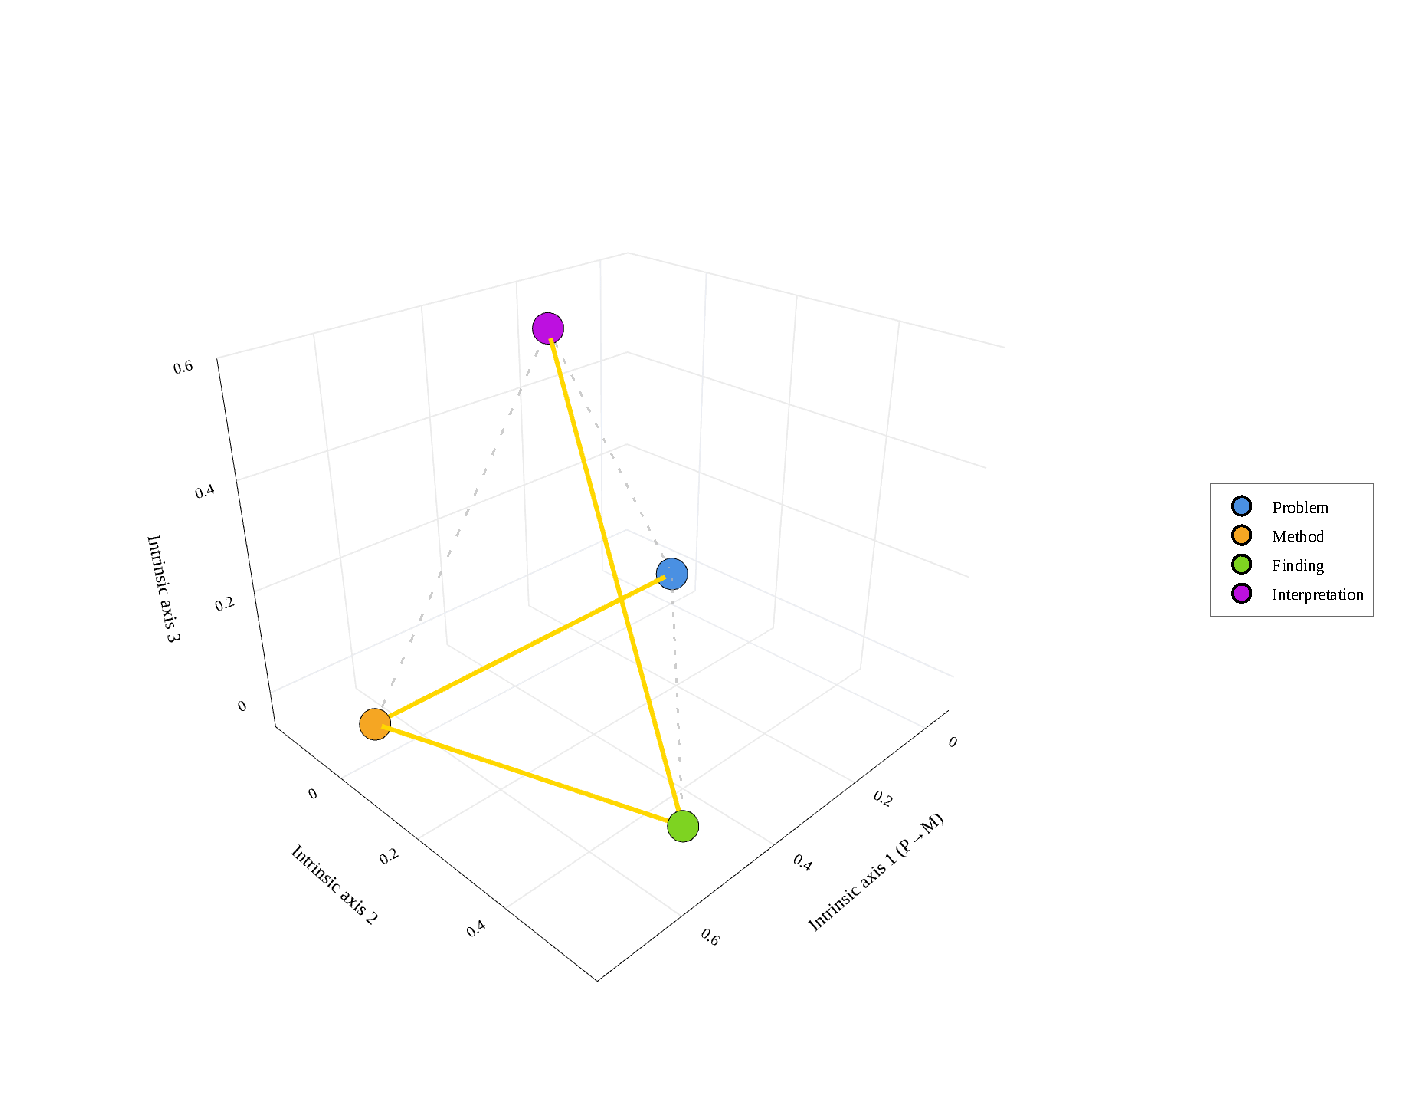
\includegraphics[width=0.72\textwidth]{figures/fig_simplex_const_subst.pdf}
\caption{Intrinsic epistemic 3-simplex $\sigma_j$ for theorem \texttt{Featherweight\_OCL.UML\_Logic.const\_subst}. Classical MDS preserves all six pairwise Euclidean distances between the four aspect embeddings ($\mathbf{p}, \mathbf{m}, \mathbf{f}, \mathbf{i}$). The sequential trajectory $P \to M \to F \to I$ is highlighted in solid gold, while non-adjacent tetrahedron edges are rendered dashed, demonstrating a non-degenerate spatial volume.}
\label{fig:simplex_const_subst}
\end{figure}

\begin{figure}[t!]
\centering
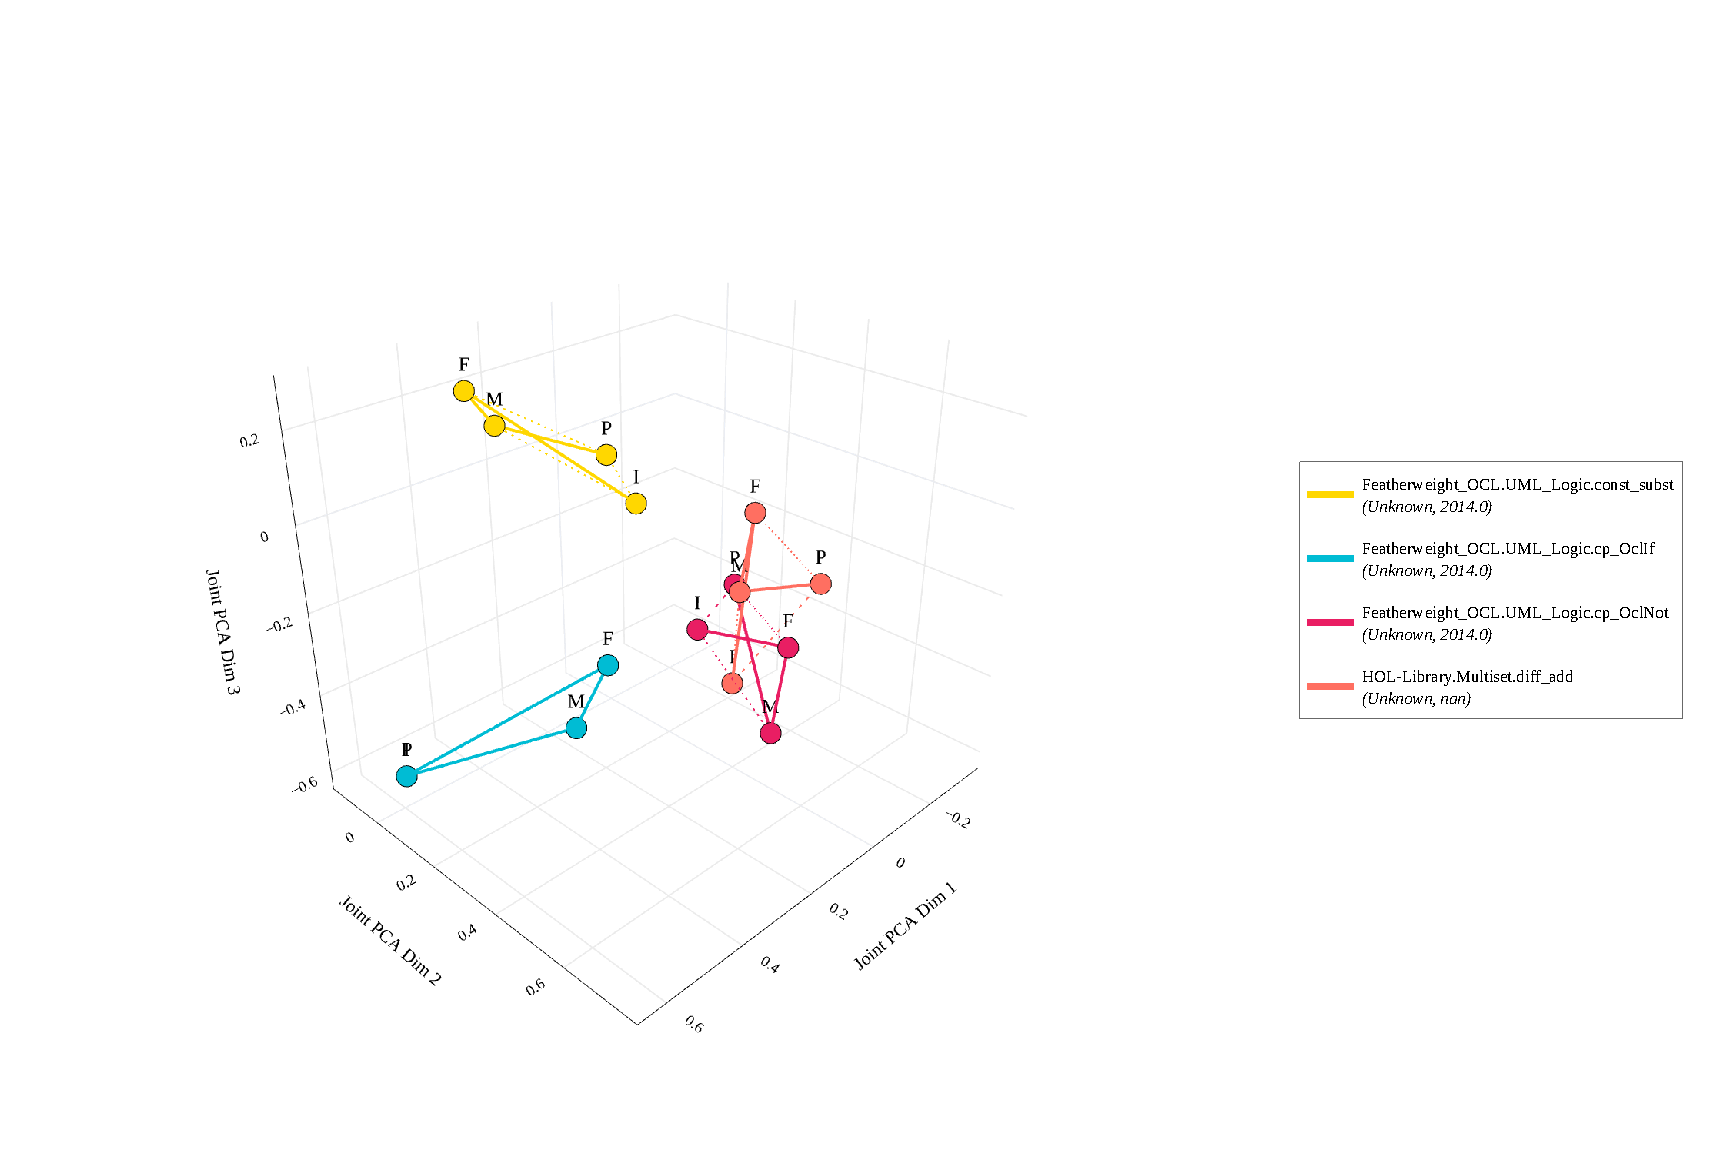
\includegraphics[width=0.85\textwidth]{figures/fig_joint_simplices.pdf}
\caption{Joint 3D PCA projection of epistemic 3-simplices across benchmark theorems. Target theorem \texttt{const\_subst} is projected alongside parent theory bridge lemmas (\texttt{cp\_OclIf}, \texttt{cp\_OclNot}) and foundational algebra lemma \texttt{Multiset.mset\_le\_incr\_right}. Distinct trajectory geometries reflect domain-specific proof strategies.}
\label{fig:joint_simplices}
\end{figure}

\begin{figure}[t!]
\centering
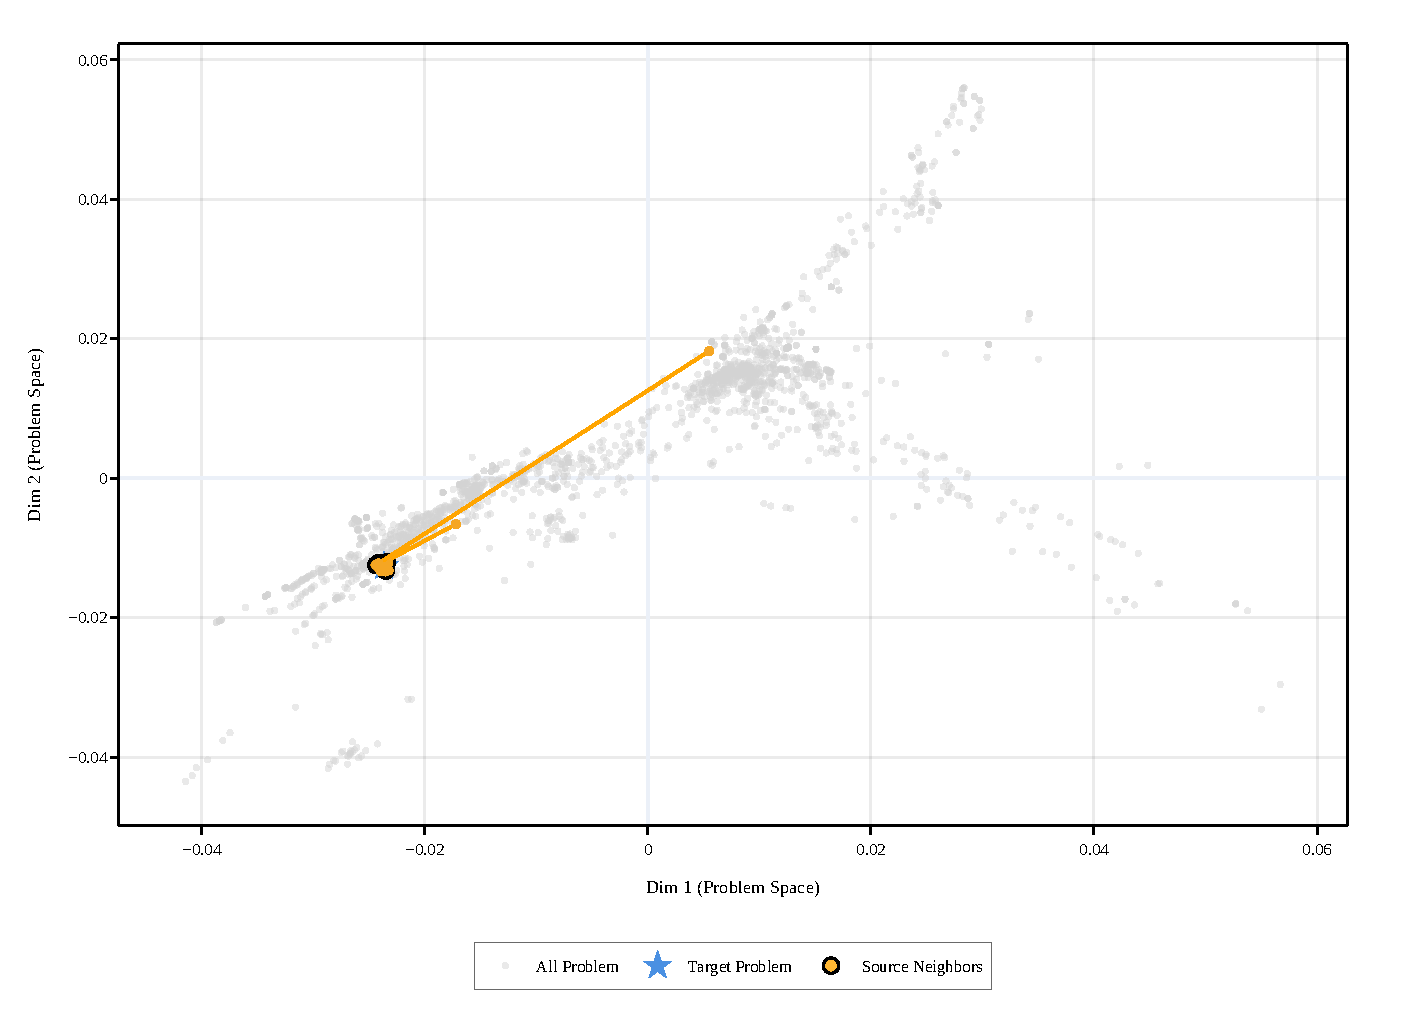
\includegraphics[width=0.72\textwidth]{figures/fig_transition_neighborhood_const_subst.pdf}
\caption{Strategic transition neighborhood $D(M \mid p)$ for theorem \texttt{const\_subst} ($k=5$ neighbors). In contrast to flat retrieval which is dominated by superficial lexical overlap, higher-order transition mapping directs search from premise representations directly into proof strategy space ($M$), retrieving parent bridge lemmas.}
\label{fig:transition_neighborhood}
\end{figure}

\begin{figure}[t!]
\centering
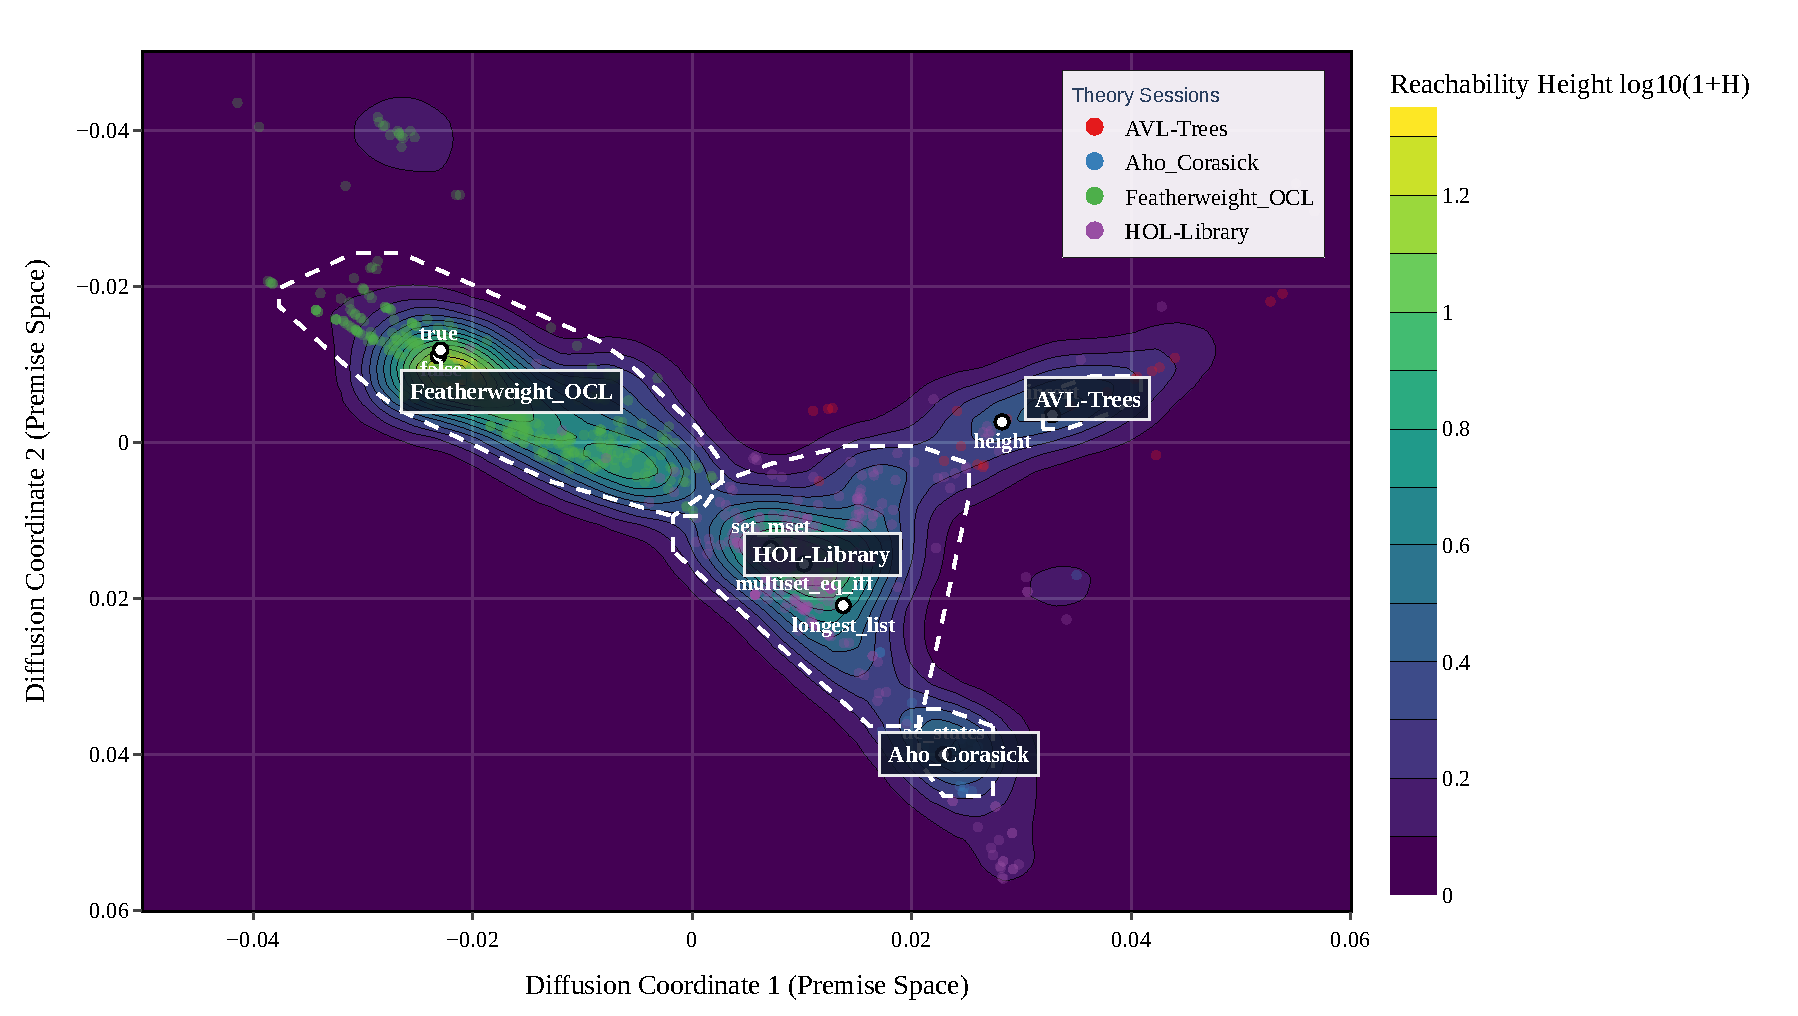
\includegraphics[width=0.82\textwidth]{figures/fig_landscape_terrain_2d.pdf}
\caption{2D Epistemic Landscape Height ($H$) contour terrain across the 1,924 benchmark theorems. Elevation contours denote downstream reachability cone size $H(v) = |\text{Reachable}_{G^T}(v)| - 1$. High topological peaks highlight foundational hubs (such as \texttt{true}, \texttt{false}, \texttt{StrongEq}) while suppressing ephemeral helper lemmas in the peripheral lowlands.}
\label{fig:landscape_terrain_2d}
\end{figure}

\begin{figure}[t!]
\centering
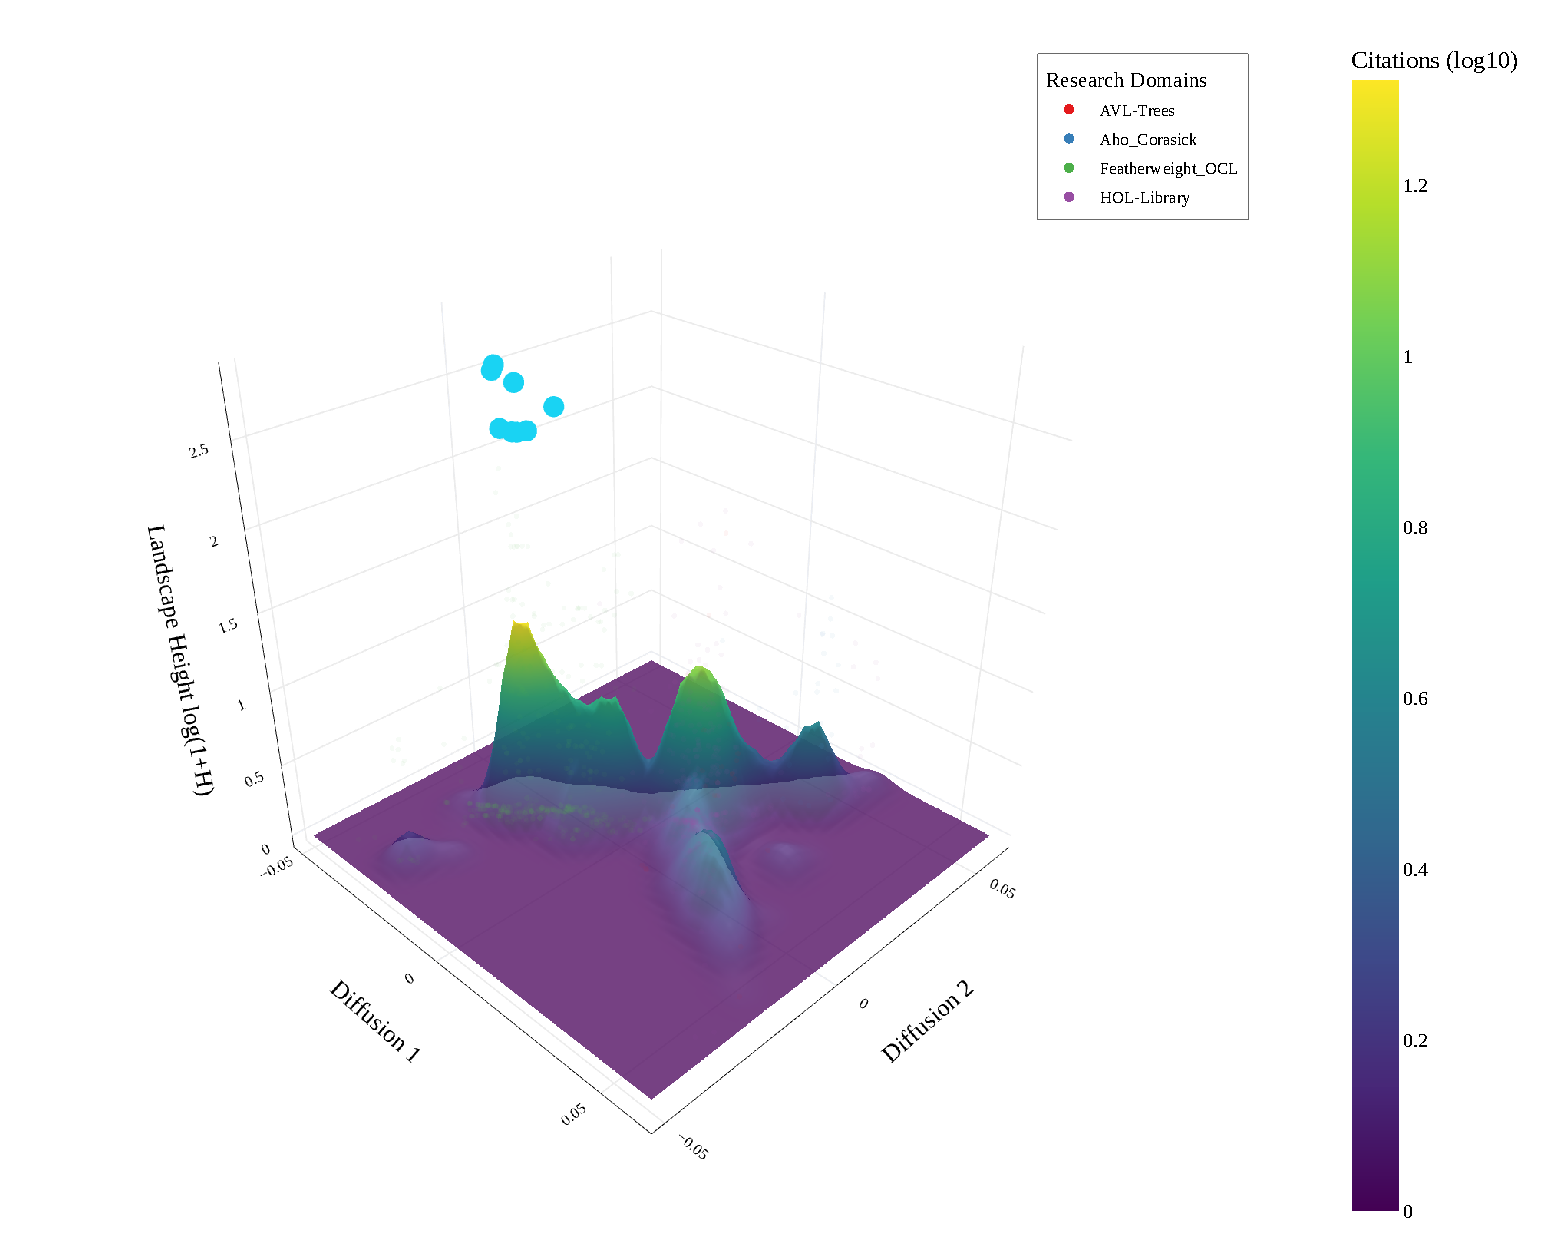
\includegraphics[width=0.82\textwidth]{figures/fig_landscape_terrain_3d.pdf}
\caption{3D continuous Epistemic Landscape over the Isabelle/HOL benchmark corpus. Topographic peaks correspond to core deductive anchors with large transitive dependency cones, guiding multi-agent reasoning toward structurally sound proof steps.}
\label{fig:landscape_terrain_3d}
\end{figure}
